\chapter{Review of acoustical and ambisonic theory}\label{chap:02_Acoustical_Theory}
In this chapter, we review relevant acoustical and ambisonic theory which will be employed throughout this thesis.
First, in \secrefthru{sec:02_Acoustical_Theory:Coordinate_System}{sec:02_Acoustical_Theory:Helmholtz_Equation}, we review the spherical Fourier-Bessel series solution to the free-field Helmholtz equation in three dimensions, which provides a frequency-domain representation of any sound pressure field in spherical coordinates.
These solutions lay the mathematical foundation for ambisonics, which we adopt to formulate the problem of virtual navigation in general, as described in \secref{sec:03_Navigation_Techniques:Problem_Formulation}, as well as to describe the implementation of each existing navigational method reviewed in \secreftwo{sec:03_Navigation_Techniques:Extrapolation_Methods}{sec:03_Navigation_Techniques:Interpolation_Methods}.

Next, in \secref{sec:02_Acoustical_Theory:Ambisonics_Encoding}, we review the so-called \textit{ambisonic encoding} equations for synthesizing ambisonics signals for point-sources and plane-waves.
These encoding equations are employed in order to simulate simple incident sound fields, as described in \chapref{chap:06_Simulation_Framework}.
These simulations are later used to comprehensively characterize the performance of various navigational methods, as described in \chaprefthru{chap:07_Characterization_Extrapolation}{chap:09_Thiergart_Comparison}.

In \secref{sec:02_Acoustical_Theory:Plane-Wave_Expansion}, we provide equations for converting between spherical-harmonic (i.e., ambisonic) and plane-wave representations of a sound field, a process which is used in the plane-wave translation method reviewed in \secref{sec:03_Navigation_Techniques:PW_Technique}.
The conversion from ambisonics to plane-wave signals is also used in the plane-wave-based ambisonics-to-binaural rendering approach described in \secref{sec:02_Acoustical_Theory:PW_Quadrature_Binaural}, as well as in the localization model proposed in \secref{sec:05_Proposed_Models:Localization_Model}.
Next, in \secref{sec:02_Acoustical_Theory:Ambisonics_Translation}, we review the spherical Fourier-Bessel translation coefficients, which are needed for the ambisonics translation method reviewed in \secref{sec:03_Navigation_Techniques:SR_Technique}.

Finally, in \secref{sec:02_Acoustical_Theory:Binaural_Rendering}, we review three linear ambisonics-to-binaural rendering approaches, one of which is employed in the listening experiments presented in \chapref{chap:05_Proposed_Models}, and all three of which have been implemented in the MATLAB toolkit described in \apxref{chap:A2_SABRE_Toolkit}.

\section{Coordinate system}\label{sec:02_Acoustical_Theory:Coordinate_System}
As is common in ambisonics, we adopt Cartesian and spherical coordinate systems in which, for a listener positioned at the origin, the $+x$-axis points forward, the $+y$-axis points to the left, and the $+z$-axis points upward.
The point $(x,y,z)$ in Cartesian coordinates is given in spherical coordinates by
\begin{equation}\label{eq:02_Acoustical_Theory:Spherical_Coordinates}
\begin{aligned}
    r &= \sqrt{x^2 + y^2 + z^2},\\
    \theta &= \arcsin \frac{z}{r},\\ % = \arcsin \mu
    \phi &= \arctan \frac{y}{x}.
\end{aligned}
\end{equation}
From this definition we see that $r$ is the (nonnegative) radial distance from the origin, $\theta \in [-\pi/2, \pi/2]$ is the elevation angle above the horizontal ($x$-$y$) plane, and $\phi \in [0, 2\pi)$ is the azimuthal angle around the vertical ($z$) axis, with $(\theta,\phi) = (0,0)$ corresponding to the $+x$ direction and $(0,\pi/2)$ to the $+y$ direction.
These variables are defined graphically in~\figref{fig:02_Acoustical_Theory:Coordinate_System}.
Conversion back to Cartesian coordinates is given by
\begin{equation}\label{eq:02_Acoustical_Theory:Cartesian_Coordinates}
\begin{aligned}
    x &= r \cos \theta \cos \phi,\\
    y &= r \cos \theta \sin \phi,\\
    z &= r \sin \theta.
\end{aligned}
\end{equation}
For a position vector $\vec{r} = (x,y,z)$, we denote the corresponding unit vector by $\hat{r} \equiv \vec{r}/r$.

\tdplotsetmaincoords{60}{120}

\pgfmathsetmacro{\rvec}{.8}
\pgfmathsetmacro{\thetavec}{30}
\pgfmathsetmacro{\phivec}{60}

\begin{figure}[t]
\centering
\begin{tikzpicture}[scale=5,tdplot_main_coords]

    \coordinate (O) at (0,0,0);
    \draw[thick,->] (0,0,0) -- (1,0,0) node[anchor=north east]{$x$};
    \draw[thick,->] (0,0,0) -- (0,1,0) node[anchor=north west]{$y$};
    \draw[thick,->] (0,0,0) -- (0,0,1) node[anchor=south]{$z$};
    \tdplotsetcoord{P}{\rvec}{\thetavec}{\phivec}
    \draw[thick,->] (O) -- (P) node[above right] {$\vec{r}$};
    \draw[dashed] (O) -- (Pxy);
    \draw[dashed] (P) -- (Pxy);
    \tdplotdrawarc{(O)}{0.2}{0}{\phivec}{anchor=north}{$\phi$}
    \tdplotsetthetaplanecoords{\phivec}
    \tdplotdrawarc[tdplot_rotated_coords]{(0,0,0)}{0.2}{90}{\thetavec}{anchor=south west}{$\theta$}

\end{tikzpicture}
\caption{Coordinate system.}\label{fig:02_Acoustical_Theory:Coordinate_System}
\end{figure}

%% Short version for papers
%As is common in ambisonics, we adopt Cartesian and spherical coordinate systems in which, for a listener positioned at the origin, the $+x$-axis points forward, the $+y$-axis points to the left, and the $+z$-axis points upward.
%Correspondingly, $r$ is the (nonnegative) radial distance from the origin, $\theta \in [-\pi/2, \pi/2]$ is the elevation angle above the horizontal ($x$-$y$) plane, and $\phi \in [0, 2\pi)$ is the azimuthal angle around the vertical ($z$) axis, with $(\theta,\phi) = (0,0)$ corresponding to the $+x$ direction and $(0,\pi/2)$ to the $+y$ direction.
%For a position vector $\vec{r} = (x,y,z)$, we denote the corresponding unit vector by $\hat{r} \equiv \vec{r}/r$.

\section{Definitions and conventions}\label{sec:02_Acoustical_Theory:Definitions}
We define the Fourier transform for acoustic signals and its corresponding inverse transform as
\begin{equation}\label{eq:02_Acoustical_Theory:Fourier_Transform}
\begin{aligned}
H(\omega) = \mathcal{F}\left[ h(t) \right] (\omega) &= \frac{1}{2 \pi} \int_{-\infty}^{\infty} h(t) e^{i \omega t}dt,\\
h(t) = \mathcal{F}^{-1}\left[ H(\omega) \right] (t) &= \int_{-\infty}^{\infty} H(\omega) e^{-i \omega t}d\omega,
\end{aligned}
\end{equation}
where $\omega$ is the angular frequency in rad/s, which is related to the temporal frequency, $f$, given in Hz, by $\omega = 2 \pi f$.
We also define the convolution operator `$\ast$' by
\begin{equation}
(h \ast g)(t) = \int_{-\infty}^{\infty} h(\tau) g(t-\tau) d\tau,
\end{equation}
which, by the convolution theorem for the Fourier transform, implies
\begin{equation}
\begin{gathered}
\mathcal{F}\left[ (h \ast g)(t) \right] (\omega) = \mathcal{F}\left[ h(t) \right] (\omega) \cdot \mathcal{F}\left[ g(t) \right] (\omega) = H(\omega) G(\omega),\\
(h \ast g)(t) = \mathcal{F}^{-1}\left[ \mathcal{F}\left[ h(t) \right] (\omega) \cdot \mathcal{F}\left[ g(t) \right] (\omega) \right] (t) = \mathcal{F}^{-1}\left[ H(\omega) G(\omega) \right] (t),
\end{gathered}
\end{equation}
where $G(\omega) = \mathcal{F}\left[ g(t) \right] (\omega)$.

Here, we use real-valued spherical harmonics, such that the spherical harmonic of degree%
\footnote{Note that ambisonics literature has long interchanged the use of the terms ``degree'' and ``order'' compared to traditional mathematical definitions of the spherical harmonics, which originate from the solutions to Laplace's equation in spherical coordinates.
Hence, the ambisonics \textit{order} actually corresponds to the mathematical \textit{degree} of the spherical harmonic.}
$l$ and order $m$ is given by~\citet[section~2.2]{Zotter2009PhD}
\begin{equation}\label{eq:02_Acoustical_Theory:Spherical_Harmonic}
Y_l^m(\theta,\phi) = N_l^{|m|} P_l^{|m|} (\sin \theta) \times
    \begin{cases}
	\cos m \phi & \textrm{for } m \geq 0,\\
	\sin |m| \phi & \textrm{for } m < 0,
    \end{cases}
\end{equation}
where $P_l^m$ is the associated Legendre polynomial of degree $l$ and order $m$, as defined in the MATLAB \texttt{legendre} function\citefooturl{MATLABlegendreURL} by
\begin{equation}
P_l^m(x) = (-1)^m (1 - x^2)^{m/2} \frac{d^m}{dx^m} P_l(x), \quad
\textrm{with} \quad
P_l(x) = \frac{1}{2^l l!} \left[ \frac{d^l}{dx^l}(x^2 - 1)^l \right],
\end{equation}
and $N_l^m$ is a normalization term which, for the orthonormal (N3D) spherical harmonics with Condon-Shortley phase,%
\footnote{Note that including Condon-Shortley phase in the normalization term cancels it in the associated Legendre term.} is given by
\begin{equation}\label{eq:02_Acoustical_Theory:Spherical_Harmonic_N3D_Normalization}
N_l^m = (-1)^m \sqrt{\frac{(2l+1)(2 - \delta_m)}{4 \pi} \frac{(l-m)!}{(l+m)!}},
\end{equation}
where $\delta_m$ is the single-argument Kronecker delta.

We define an inner product on the unit sphere by
\begin{equation}
\left< h, g \right> \equiv \int_{\phi=0}^{2 \pi} \int_{\theta=-\frac{\pi}{2}}^{\frac{\pi}{2}} h(\theta,\phi) \overline{g(\theta,\phi)} \cos \theta d\theta d\phi,
\end{equation}
where $\overline{g}$ denotes the complex conjugate of $g$.
Therefore, the inner product of any two N3D-normalized spherical harmonic functions is given by
\begin{equation}
\left< Y_l^m, Y_{l'}^{m'} \right> = \delta_{l,l'} \delta_{m,m'},
\end{equation}
where $\delta_{m,m'}$ is the Kronecker delta (with two arguments),
and the squared norm of any spherical harmonic function is given by
\begin{equation}
\|Y_l^m\|^2 \equiv \left< Y_l^m, Y_l^m \right> = 1.
\end{equation} % Follows from inner product
Consequently, we see that the N3D spherical harmonics form an orthonormal basis on the unit sphere.

A commonly-used alternative is the Schmidt seminormalized (SN3D) spherical harmonic normalization convention (again with Condon-Shortley phase), given by \citep{Nachbar2011}
\begin{equation}\label{eq:02_Acoustical_Theory:Spherical_Harmonic_SN3D_Normalization}
N_l^m = (-1)^m \sqrt{\frac{2 - \delta_m}{4 \pi} \frac{(l-m)!}{(l+m)!}}.
\end{equation}
With the same choice of inner product, the inner product of any two spherical harmonic functions is given by
\begin{equation}
\left< Y_l^m, Y_{l'}^{m'} \right> = \frac{\delta_{l,l'} \delta_{m,m'}}{2l+1}
\end{equation}
and the squared norm of any spherical harmonic function is given by
\begin{equation}
\|Y_l^m\|^2 = \frac{1}{2l+1}.
\end{equation} % Follows from inner product
Consequently, we note that the SN3D spherical harmonics are \textit{not} orthonormal on the unit sphere, but they do yield an orthogonal basis.

We also adopt the ambisonics channel numbering (ACN) convention~\citep{Nachbar2011} such that for a spherical harmonic function of degree $l \in [0,\infty)$ and order $m \in [-l,l]$, the ACN index $n$ is given by
\begin{equation}\label{eq:02_Acoustical_Theory:AmbOrder_To_ACN}
n = l (l + 1) + m
\end{equation}
and we denote the spherical harmonic function by $Y_n \equiv Y_l^m$.
Correspondingly, for ACN index $n$, the spherical harmonic degree and order are given by
\begin{equation}\label{eq:02_Acoustical_Theory:ACN_To_AmbOrder}
\begin{aligned}
l &= \left\lfloor \sqrt{n} \right\rfloor,\\
m &= n - l (l + 1),
\end{aligned}
\end{equation}
where $\lfloor \cdot \rfloor$ denotes rounding down to the nearest integer (i.e., the ``floor'' function).

Alternative ordering and normalization schemes, such as Furse-Malham (``FuMa'') and ``MaxN'', are discussed by \citet[and references therein]{Carpentier2017}.

\section{Helmholtz equation and region of validity}\label{sec:02_Acoustical_Theory:Helmholtz_Equation}
We define the \textit{acoustic potential field} $\psi$ as the Fourier transform of the acoustic pressure field, such that, in the \textit{free-field} (i.e., in a region free of sources and scattering bodies), the acoustic potential field satisfies the homogeneous Helmholtz equation,
\begin{equation}\label{eq:02_Acoustical_Theory:Helmholtz_Equation}
\left( \nabla^2 + k^2 \right) \psi(k,\vec{r}) = 0,
\end{equation}
where $\nabla^2$ is the Laplace operator, $k = \omega / c$ is the angular wavenumber, and $c \approx 343$~m/s is the speed of sound.

Depending on our region of interest, we may impose different boundary conditions on the problem in order to ensure that our solution for the acoustic potential field is physically possible.
For example, for an exterior (free-field) region of interest, all sources and obstacles must exist within a spherical region centered on the origin and of some finite radius, $R$.
Consequently, the solution must satisfy the Sommerfeld radiation condition \citep[section 2.1.1]{Zotter2009PhD}, which can be written as
\begin{equation}
\lim_{r\to\infty} \left[ r \left( \frac{\partial}{\partial r} - i k \right) \psi (k,\vec{r}) \right] = 0.
\end{equation}
Although multiple physical interpretations of this condition exist (cf.~\citet[appendix A]{Zotter2009PhD}, \citet[section 4-5]{Pierce1994}), essentially it states that power must only be radiating away from sources located near the origin, rather than arriving from infinity and being destroyed \citep{WikiSommerfeldURL}.
In this case, we must choose singular, radiating basis solutions to the Helmholtz equation, which are given by $h_l(kr) Y_n(\hat{r})$, where $h_l$ is the (outgoing) spherical Hankel function of the first kind and of order $l$, and $Y_n$ is the spherical harmonic for ACN index $n$ \citep[section 6.7]{Williams1999}.
The interested reader is referred to the works of \citet{Zotter2009PhD,Williams1999} for more detailed discussions of such exterior problems.

For an interior region of interest, where all sources exist beyond some finite radius $R$ away from the origin, we require that the solution be finite in magnitude everywhere inside that region, i.e., $|\psi| < \infty,~\forall r < R$.
In this case, we must choose regular (i.e., not singular) basis solutions to the Helmholtz equation, which are given by $j_l(kr) Y_n(\hat{r})$, where $j_l$ is the spherical Bessel function of order $l$ \citep[section 6.8]{Williams1999}.
%These solutions are only valid under free-field conditions, and can be used to describe the acoustic potential in an interior region, that is, for $r < R$, where $R$ is a finite distance .
%So that the region remains source- and obstacle-free, $R$ is typically taken to be the distance of the nearest source or scattering body to the origin.
This spherical interior region where $r < R$ is the so-called \textit{region of validity}, which is illustrated in \figref{fig:02_Acoustical_Theory:Region_of_Validity}.

% Diagram of source/mic positions
\begin{figure}[t]
\centering
  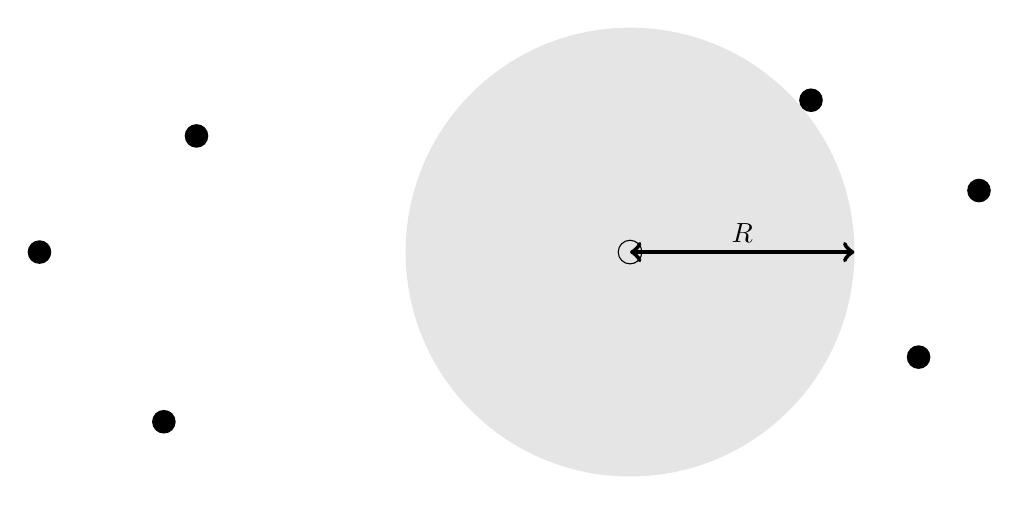
\begin{tikzpicture}[scale=3]
% Parameters
\def\radius{1};
\def\validR{0.95};
\def\sourceR{1-\validR}

\pgfmathsetmacro\evalX{cos(140)*\radius}
\pgfmathsetmacro\evalY{sin(140)*\radius}

\pgfmathsetmacro\sourceXa{cos(-20)*1.3*\radius}
\pgfmathsetmacro\sourceYa{sin(-20)*1.3*\radius}

\pgfmathsetmacro\sourceXb{cos(10)*1.5*\radius}
\pgfmathsetmacro\sourceYb{sin(10)*1.5*\radius}

\pgfmathsetmacro\sourceXc{cos(200)*2.1*\radius}
\pgfmathsetmacro\sourceYc{sin(200)*2.1*\radius}

\pgfmathsetmacro\sourceXd{cos(180)*2.5*\radius}
\pgfmathsetmacro\sourceYd{sin(180)*2.5*\radius}

\pgfmathsetmacro\sourceXe{cos(165)*1.9*\radius}
\pgfmathsetmacro\sourceYe{sin(165)*1.9*\radius}

\pgfmathsetmacro\sourceXf{cos(40)*\radius}
\pgfmathsetmacro\sourceYf{sin(40)*\radius}

\fill [color=black,opacity=0.1] (0,0) circle (\validR*\radius);

%\node at (0,0){$\times$};
\draw [color=black] (0,0) circle (\sourceR*\radius);
\draw[ultra thick,<->] (0,0) -- (\validR*\radius,0);
\node[above] at (0.5*\validR*\radius,0){$R$};

% Source positions
\fill [color=black] (\sourceXa,\sourceYa) circle (\sourceR*\radius);
\fill [color=black] (\sourceXb,\sourceYb) circle (\sourceR*\radius);
\fill [color=black] (\sourceXc,\sourceYc) circle (\sourceR*\radius);
\fill [color=black] (\sourceXd,\sourceYd) circle (\sourceR*\radius);
\fill [color=black] (\sourceXe,\sourceYe) circle (\sourceR*\radius);
\fill [color=black] (\sourceXf,\sourceYf) circle (\sourceR*\radius);
\end{tikzpicture}
  \caption[Diagram of the region of validity for an interior free-field region.]{
  Diagram of the region of validity for a free-field spherical Fourier-Bessel expansion.
  The empty circle indicates the expansion center,
  the filled circles indicate source positions,
  and the shaded disk indicates the region of validity.
  The radius of the region of validity is equal to $R$, the distance of the nearest source from the expansion center.}
  \label{fig:02_Acoustical_Theory:Region_of_Validity}
\end{figure}

Inside this region, any acoustic potential field can be written as an infinite sum of regular solutions, known as a spherical Fourier-Bessel series expansion, given by \citep[chapter 2]{GumerovDuraiswami2005}
\begin{equation}\label{eq:02_Acoustical_Theory:Infinite_Order_Expansion}
\psi(k,\vec{r}) = \sum_{n=0}^{\infty} 4\pi (-i)^l A_n(k) j_l(kr) \frac{Y_n(\hat{r})}{\|Y_n\|^2},
\end{equation}
where $A_n$ are the corresponding (frequency-dependent) expansion coefficients and we have, without loss of generality, factored out $(-i)^l$ to ensure conjugate-symmetry in each $A_n$, making each ambisonics signal (i.e., the inverse Fourier transform of $A_n$) real-valued for a real pressure field.
Note that this expansion need not be taken about the origin, but instead can be taken about any arbitrary expansion center, in which case the region of validity refers to a spherical free-field region centered about that point.
In practice, this expansion is truncated to a finite order $L$ (i.e., $l \in [0,L]$), yielding $N = (L + 1)^2$ terms,
\begin{equation}\label{eq:02_Acoustical_Theory:Finite_Order_Expansion}
\psi(k,\vec{r}) = \sum_{n=0}^{N - 1} 4\pi (-i)^l A_n(k) j_l(kr) \frac{Y_n(\hat{r})}{\|Y_n\|^2}.
\end{equation}

\section{Ambisonics encoding equations}\label{sec:02_Acoustical_Theory:Ambisonics_Encoding}
For a point-source that generates an impulse at $t = t_0$ and is located at $\vec{s}_0$, the emitted pressure field (impulse response) is given by
\begin{equation}
p(t,\vec{r}) = \frac{2 \pi}{\left\| \vec{r} - \vec{s}_0 \right\|} \cdot \delta \left( (t-t_0) - \frac{\left\| \vec{r} - \vec{s}_0 \right\|}{c} \right),
\end{equation}
where $\|\cdot\|$ denotes the $\ell^2$ norm (Euclidean distance) of a vector.
Taking the Fourier transform yields the acoustic potential field (transfer function) of that point-source, given by \citep[Eq.~(6.73)]{Williams1999}
\begin{equation}\label{eq:02_Acoustical_Theory:PointSource}
\psi(k,\vec{r}) = \frac{e^{i k \left\| \vec{r} - \vec{s}_0 \right\|}}{\left\| \vec{r} - \vec{s}_0 \right\|} e^{i k c t_0} = i k \cdot h_0 (k \left\| \vec{r} - \vec{s}_0 \right\| ) \cdot e^{i k c t_0}.
\end{equation} % Confirmed in Mathematica
%where, in general, $h_l$ is the (outgoing) spherical Hankel function of the first kind and of order $l$.
The spherical Fourier-Bessel expansion of this expression (ignoring the time delay term) is given by~\citep[Eq.~(8.22)]{Williams1999}
\begin{align}
\frac{e^{i k \left\| \vec{r} - \vec{s}_0 \right\|}}{\left\| \vec{r} - \vec{s}_0 \right\|} &= 4 \pi i k \sum_{l=0}^{\infty} j_l(k r) h_l(k s_0) \sum_{m=-l}^{l} Y_l^m (\hat{s}_0) \frac{Y_l^m (\hat{r})}{\|Y_l^m\|^2} \\
	&= \sum_{n=0}^{\infty} \left[ i^{l+1} k h_l(k s_0) Y_n (\hat{s}_0) \right] 4 \pi (-i)^l j_l(k r) \frac{Y_n (\hat{r})}{\|Y_n\|^2},
\end{align} % Confirmed in MATLAB
where we have assumed $r < s_0$ in order for $\vec{r}$ to be within the region of validity.
Thus, the ambisonics encoding filters for this point source are given by
\begin{equation}\label{eq:02_Acoustical_Theory:PointSource_An}
A_n(k) = \underbrace{i^{l+1} k h_l(k s_0)}_{\text{distance coding}} \underbrace{Y_n (\hat{s}_0)}_{\text{panning}} \underbrace{ \vphantom{ Y_n (\hat{s}_0) } e^{i k c t_0}}_{\text{delay}}.
\end{equation}

%The ambisonics encoding filters for a point source located at $\vec{s}_0$ are given in the frequency domain by~\citep[Eq.~(10)]{Poletti2005}
%\begin{equation}\label{eq:02_Acoustical_Theory:PointSource_An}
%A_n(k) = i^{l+1} k h_l(k s_0) Y_n (\hat{s}_0),
%\end{equation}
%where $h_l$ is the (outgoing) spherical Hankel function of order $l$.

For a plane-wave source located in the direction $\hat{s}_0$ (and propagating in the direction $-\hat{s}_0$), the pressure field is given by
\begin{equation}
p(t,\vec{r}) = 2 \pi \cdot \delta \left( (t-t_0) + \frac{\hat{s}_0 \cdot \vec{r}}{c} \right),
\end{equation}
where now $t = t_0$ indicates the time at which the impulse reaches the origin ($r = 0$).
Taking the Fourier transform yields the acoustic potential field of this plane-wave, given by \citep[Eq.~(2.24), with $\vec{k} = -k\hat{s}_0$]{Williams1999}
\begin{equation}
\psi(k,\vec{r}) = e^{-i k \hat{s}_0 \cdot \vec{r}} e^{i k c t_0}.
\end{equation} % Confirmed in Mathematica
The spherical Fourier-Bessel expansion of this expression (ignoring the time delay term) is given by~\citep[Eq.~(6.175)]{Williams1999}
\begin{align}
e^{-i k \hat{s}_0 \cdot \vec{r}} &= 4 \pi \sum_{l=0}^{\infty} i^l j_l(k r) \sum_{m=-l}^{l} Y_l^m (-\hat{s}_0) \frac{Y_l^m (\hat{r})}{\|Y_l^m\|^2}\\
	&= \sum_{n=0}^{\infty} Y_n (\hat{s}_0) 4 \pi (-i)^l j_l(k r) \frac{Y_n (\hat{r})}{\|Y_n\|^2} ,
\end{align} % Confirmed in MATLAB
since $Y_l^m (-\hat{s}_0) = (-1)^l Y_l^m (\hat{s}_0)$.
Thus, the ambisonics encoding filters for this plane-wave source are given by
\begin{equation}\label{eq:02_Acoustical_Theory:PlaneSource_An}
A_n(k) = \underbrace{Y_n (\hat{s}_0)}_{\text{panning}} \underbrace{ \vphantom{ Y_n (\hat{s}_0) } e^{i k c t_0}}_{\text{delay}}.
\end{equation}

%For a plane-wave source, the ambisonics encoding filters are given by
%\begin{equation}\label{eq:02_Acoustical_Theory:PlaneSource_An}
%A_n(k) = Y_n (\hat{s}_0).
%\end{equation}

\subsection{Near-field amplification and compensation}\label{sec:02_Acoustical_Theory_Nearfield_Compensation}
Consider the following order-dependent function, $F_l(\zeta)$, given by
\begin{equation}\label{eq:02_Acoustical_Theory:Fl_zeta}
F_l(\zeta) = \zeta l h_l (\zeta l).
\end{equation}
This family of functions is plotted in \figref{fig:02_Acoustical_Theory:Nearfield_Amplification}.
From this figure, we note that amplification occurs below $\zeta = 1$, with the slope of the amplification increasing with increasing $l$.

% Near-field amplification
\begin{figure}[t]
\centering
  \includegraphics[width = 0.6\textwidth]{02_acoustical_theory/figures/nearfield_amplification.eps}
  \caption[Magnitudes of the family of functions given in \eqnref{eq:02_Acoustical_Theory:Fl_zeta}.]{
  Magnitudes of the family of functions given in \eqnref{eq:02_Acoustical_Theory:Fl_zeta} for increasing values of $l$ from $l = 1$ (black curve) to $6$ (lightest gray).
  If the nondimensional wavenumber $k s_0 / l$ is substituted for $\zeta$, then these curves illustrate the near-field amplification introduced when encoding a point-source into ambisonics (see \eqnref{eq:02_Acoustical_Theory:Nearfield_Amplification} and cf.~\citet[Fig.~4]{Daniel2003b}).}
  \label{fig:02_Acoustical_Theory:Nearfield_Amplification}
\end{figure}

If we let $\zeta = k s_0 / l$, we can relate this function to the distance-coding term of the point-source encoding filters (as given in \eqnref{eq:02_Acoustical_Theory:PointSource_An}) by
\begin{equation}\label{eq:02_Acoustical_Theory:Nearfield_Amplification}
\left| s_0 \frac{A_n (k)}{Y_n (\hat{s}_0)} \right| = \left| k s_0 h_l (k s_0) \right| = \left| F_l \left( \frac{k s_0}{l} \right) \right|,
\end{equation}
where $|\cdot|$ denotes the absolute value (or modulus or magnitude) of the argument.
From this relationship, we see that increasing (or decreasing) the source distance $s_0$ has two effects on the resulting ambisonics signals:
\begin{enumerate}
\item the overall amplitude of each ambisonics signal decreases (increases), and
\item the frequency below which the amplification occurs decreases (increases).
\end{enumerate}
In particular, the ambisonics signals are amplified at frequencies below $k = l / s_0$ (cf.~\citep[section 2.1]{Daniel2003b}).

To prevent excessive low-frequency amplification from this effect, we define for all ambisonics orders $l \in [1, L_\textrm{in}]$, an order-dependent, zero-phase high-pass Butterworth filter, the frequency response of which is given by
\begin{equation}\label{eq:02_Acoustical_Theory:NearField_HPF}
H_l(f) = 1 - \frac{1}{\sqrt{1 + \left( \frac{f}{f_l} \right)^l}},
\end{equation}
where $f_l$ is the corner frequency of the $l^\textrm{th}$ filter,
which, unless stated otherwise, we choose to be $f_l = (200 \times l)$~Hz.

As shown above, the frequency at which the near-field amplification occurs increases as the distance between the source and microphone decreases.
However, the compensation filters given in~\eqnref{eq:02_Acoustical_Theory:NearField_HPF} are independent of source position, which will lead to excessive low-frequency amplification (due to insufficient compensation) at small source distances and excessive low-frequency attenuation at large source distances.
The plots in \figref{fig:02_Acoustical_Theory:Nearfield_Compensation} illustrate this effect for $s_0 = 0.05, 1$~m.
This approach, while inexact, is representative of practical reality since, in general, the source position(s) may be unknown.
Indeed, the Eigenmike by mh acoustics uses distance-independent compensation filters \citep[section 4.3]{EigenUnitsManual2018}.
(In the experimental validation presented in \chapref{chap:10_Experimental_Validation}, we use distance-independent compensation filters to match those of the Eigenmike.)

\begin{figure}[t]
    \centering
    \begin{subfigure}[b]{0.49\textwidth}
        \includegraphics[width=\textwidth]{02_acoustical_theory/figures/nearfield_compensation_5cm.eps}
        \caption{$s_0 = 0.05$~m}
    \end{subfigure}
    \hfill
    \begin{subfigure}[b]{0.49\textwidth}
        \includegraphics[width=\textwidth]{02_acoustical_theory/figures/nearfield_compensation_100cm.eps}
        \caption{$s_0 = 1$~m}
    \end{subfigure}
\caption[Residual near-field amplification after compensation.]{
Residual near-field amplification for two different source distances after compensation with the Butterworth high-pass filter (see \eqnref{eq:02_Acoustical_Theory:NearField_HPF}).
The magnitude spectra have been multiplied by $s_0$ in order to remove the vertical offset caused by the overall distance attenuation.}
\label{fig:02_Acoustical_Theory:Nearfield_Compensation}
\end{figure} %%NOTE%% vertical axis label is too complicated: |A H| s or something

\section{Plane-wave decomposition}\label{sec:02_Acoustical_Theory:Plane-Wave_Expansion}
Given spherical Fourier-Bessel expansion coefficients, $A_n$, the so-called \textit{signature function}, $\mu$, in the direction $\hat{v}_q$ is given by~\citep[section~2.3.3]{GumerovDuraiswami2005}
\begin{equation}\label{eq:02_Acoustical_Theory:A2mu}
\mu(k,\hat{v}_q) = \sum_{n=0}^{N-1} A_n(k) \frac{Y_n(\hat{v}_q)}{\left\|Y_n\right\|^2}.
\end{equation}
This computation of the signature function is often referred to as \textit{modal beamforming},%
\footnote{This is as opposed to \textit{delay-and-sum beamforming}, in which the appropriately-delayed signals from each individual microphone capsule in an array are summed to isolate the signals from a desired incident direction (which will be added in-phase) while cancelling signals arriving from other directions.}
as the process amounts to an isolation of the sound coming from the direction $\hat{v}_q$ (the so-called ``look direction'') via a linear combination of the different spherical ``modes'' of the sound field (cf.~\citet{HahnSpors2015b,Spors2012}).

The signature function represents the coefficients of a plane-wave decomposition of the sound field, such that the potential field can be approximately reconstructed using a finite number of plane-waves.%
\footnote{Alternatively, the signature function can be computed using a pseudoinverse of a matrix of spherical harmonics, as described in \eqnref{eq:02_Acoustical_Theory:A2mu_Pinv}.}
Assuming that the spherical Fourier-Bessel expansion was taken about the origin, this reconstructed potential field is given by
\begin{equation}\label{eq:02_Acoustical_Theory:PW_Quadrature_Rendered_Field}
\psi(k,\vec{r}) \approx \sum_{q=1}^Q w_q \mu(k,\hat{v}_q) e^{-i k \hat{v}_q \cdot \vec{r}},
\end{equation}
where $Q$ is the number of plane-wave terms, $\hat{v}_q$ is the source direction of the $q^\text{th}$ term, and $w_q$ is its quadrature weight, which is dependent on the chosen grid of directions.
By convention, we assume $\sum_{q=1}^Q w_q \approx 4 \pi$, and typically require that $w_q \neq 0,~\forall q \in [1, Q]$.

The signature function can be converted back into ambisonics signals, given by
\begin{equation}\label{eq:02_Acoustical_Theory:mu2A_Quadrature}
A_n(k) = \sum_{q=1}^{Q} w_q \mu(k,\hat{v}_q) Y_{n}(\hat{v}_q),
\end{equation}
where we have essentially encoded the sum of $Q$ plane-wave signals via \eqnref{eq:02_Acoustical_Theory:PlaneSource_An}.

\section{Ambisonics translation coefficients}\label{sec:02_Acoustical_Theory:Ambisonics_Translation}
Let $R_n(k, \vec{r})$ denote the spherical Fourier-Bessel basis functions defined in \secref{sec:02_Acoustical_Theory:Helmholtz_Equation} (see \eqnref{eq:02_Acoustical_Theory:Infinite_Order_Expansion}) and given by
\begin{equation}\label{eq:02_Acoustical_Theory:Basis_Functions}
R_n(k, \vec{r}) = 4\pi (-i)^l j_l(kr) \frac{Y_n(\hat{r})}{\|Y_n\|^2}.
\end{equation}
It can be shown that these basis functions can be translated along the vector $\vec{r}_0$ by \citep[Eq.~(3.2.1)]{GumerovDuraiswami2005}
\begin{equation}\label{eq:02_Acoustical_Theory:Translated_Basis_Functions}
R_n(k, \vec{r} + \vec{r}_0) = \sum_{n' = 0}^\infty T_{n,n'}(k,\vec{r}_0) R_{n'}(k, \vec{r}),
\end{equation}
where $T_{n,n'}$ are the so-called \textit{translation coefficients}.
Integral forms of these translation coefficients as well as fast recurrence relations for computing them are given by \citet[section~3.2]{GumerovDuraiswami2005} and \citet[chapter 3]{Zotter2009PhD}.
Additionally, a distilled algorithm for computing these coefficients is given by \citet{TylkaChoueiri2019a}, which is reproduced in \apxref{chap:A1_Navigation_Filters} of the present thesis.

Now let us consider two sets of spherical Fourier-Bessel expansion coefficients for the same sound field: $B_n$, which describe the sound field for an expansion about the origin, and $A_{n'}$, which do the same for an expansion about $\vec{r}_0$.
By \eqnref{eq:02_Acoustical_Theory:Infinite_Order_Expansion}, the acoustic potential field is given by
\begin{equation}
\psi(k,\vec{r} + \vec{r}_0) = \sum_{n' = 0}^\infty A_{n'}(k) R_{n'}(k, \vec{r}) = \sum_{n = 0}^\infty B_n(k) R_n(k, \vec{r} + \vec{r}_0).
\end{equation}
Substituting \eqnref{eq:02_Acoustical_Theory:Translated_Basis_Functions} into the above equation yields
\begin{equation}
\sum_{n' = 0}^\infty A_{n'}(k) R_{n'}(k, \vec{r}) = \sum_{n = 0}^\infty B_n(k) \left[ \sum_{n' = 0}^\infty T_{n,n'}(k,\vec{r}_0) R_{n'}(k, \vec{r}) \right].
\end{equation}
Rearranging and interchanging the order of the summations%
\footnote{Note that this is possible when the summations converge absolutely and uniformly \citep[section 3.1.1]{GumerovDuraiswami2005}, which is likely the case since the expression necessarily converges to a finite $\psi$ for real sound fields.
In any case, since in practice these summations will be truncated at a finite order, swapping the order becomes trivial.}
reveals
\begin{align}
\sum_{n' = 0}^\infty A_{n'}(k) R_{n'}(k, \vec{r}) &= \sum_{n' = 0}^\infty \left[ \sum_{n = 0}^\infty T_{n,n'}(k,\vec{r}_0) B_n(k) \right] R_{n'}(k, \vec{r}), \\
\implies A_{n'}(k) &= \sum_{n = 0}^\infty T_{n,n'}(k, \vec{r}_0) B_n(k).
\end{align}

In practice, we have only a truncated series expansion of the sound field, with measured coefficients $B_n$ up to order $L$, such that we compute
\begin{equation}\label{eq:02_Acoustical_Theory:Translated_Expansion_Coefficients}
A_{n'}(k) = \sum_{n = 0}^{N-1} T_{n,n'}(k, \vec{r}_0) B_n(k),
\end{equation}
where $N = (L + 1)^2$.
This translation process is illustrated in \figref{fig:03_Navigation_Techniques:Problem_Formulation} for an arbitrary original expansion center, $\vec{u}$.
Note that the translated expansion coefficients $A_{n'}$ can be computed to an arbitrary order $L'$, with $N' = (L' + 1)^2$ terms.

In matrix form, we can write \eqnref{eq:02_Acoustical_Theory:Translated_Expansion_Coefficients} as
\begin{equation}\label{eq:02_Acoustical_Theory:Translated_Expansion_Coefficients_Matrix}
\mathbf{a}(k) = \left( \mathbf{T}(k, \vec{r}_0) \right)^\text{T} \cdot \mathbf{b}(k),
\end{equation}
where $(\cdot)^\text{T}$ denotes the transpose of the argument and, omitting dependencies,
\begin{equation}\label{eq:02_Acoustical_Theory:Expansion_Coefficients_Vectors}
\mathbf{a} = 
    \left[ \begin{array}{c}
    A_0\\
    A_1\\
    \vdots\\
    A_{N'-1}
    \end{array} \right]
,\quad
\mathbf{b} = 
    \left[ \begin{array}{c}
    B_0\\
    B_1\\
    \vdots\\
    B_{N-1}
    \end{array} \right],
\end{equation}
and
\begin{equation}\label{eq:02_Acoustical_Theory:Translation_Matrix}
\mathbf{T}_{(N \times N')} = 
    \left[ \begin{array}{cccc}
    T_{0,0} & T_{0,1} & \cdots & T_{0,N'-1}\\
    T_{1,0} & T_{1,1} & \cdots & T_{1,N'-1}\\
    \vdots & \vdots & \ddots & \vdots\\
    T_{N-1,0} & T_{N-1,1} & \cdots & T_{N-1,N'-1}
    \end{array} \right].
\end{equation}
An algorithm to compute this matrix via recurrence relations is given in~\apxref{chap:A1_Navigation_Filters}.

\section{Rendering (decoding) ambisonics to binaural}\label{sec:02_Acoustical_Theory:Binaural_Rendering}
Generally, binaural decoding of ambisonics aims to generate the appropriate binaural signals for a listener at a point (with any orientation) in a recorded (or synthesized) sound field,
such that the resulting perception of the sound field is identical to that which would have occurred in the real sound field.
At the origin, this task may be accomplished by:
\begin{enumerate}
\item decoding the ambisonics signals to a fixed set of virtual loudspeakers and filtering each loudspeaker's signal by the appropriate HRTF \citep{McKeagMcGrath1996,Noisternig2003a},
\item transforming the ambisonics signals into a plane-wave expansion of the sound field and filtering each plane-wave term by the appropriate HRTF \citep{Duraiswami2005a,MenziesAlAkaidi2007b}, 
\item using a spherical-harmonic decomposition of the listener's HRTFs to filter each ambisonics signal directly \citep{RafaelyAvni2010,Bernschutz2014}, or
\item decomposing the (typically first-order only) ambisonics signals into directional (and diffuse) components using non-linear, parametric techniques (e.g., HARPEX, DirAC) and filtering each component by the appropriate HRTF \citep{Laitinen2008,BergeBarrett2010b}.
\end{enumerate}
In this section, we review the first three approaches listed above.
A corresponding MATLAB toolkit developed by the present author which implements these first three approaches is presented in \apxref{chap:A2_SABRE_Toolkit}.

\subsection{Virtual ambisonics}\label{sec:02_Acoustical_Theory:VA_Binaural}
Generally, the ambisonics decoding matrix, $\mathbf{D}$, which is typically time- and frequency-independent,%
\footnote{Although two- or multi-band decoders are commonly used, the decoder matrix for each sub-band is typically time-independent \citep{Heller2012}.}
determines the loudspeaker signals, $g_q$, given by
\begin{equation}\label{eq:02_Acoustical_Theory:Ambisonics_Decoding}
\mathbf{g}(t) = 
\begin{bmatrix}
g_{1}(t) \\ g_{2}(t) \\ \vdots \\ g_{Q}(t)
\end{bmatrix}
 = \mathbf{D} \cdot 
\begin{bmatrix}
a_{0}(t) \\ a_{1}(t) \\ \vdots \\ a_{N-1}(t)
\end{bmatrix}
 = \mathbf{D} \cdot \mathbf{a}(t),
\end{equation}
where $Q$ is the number of loudspeakers and $a_n$ is the $n^\text{th}$ ambisonics signal.
Methods of calculating the decoding matrix have been extensively researched and it is outside of the scope of this thesis to discuss them in detail.
Briefly, the decoding matrix attempts to use all available loudspeakers to create a perceptually-accurate reproduction the recorded sound field \citep{Heller2012}.

Following traditional ambisonic theory,
we consider the ambisonics signals produced at the center of the loudspeaker array
in response to the loudspeaker signals, given by
\begin{equation}
a_n(t) = \sum_{q=1}^{Q} Y_{n}(\hat{v}_q) g_q(t).
\end{equation}
(Note that this effectively treats the loudspeakers as plane-wave sources via \eqnref{eq:02_Acoustical_Theory:PlaneSource_An}.)
Equivalently, in matrix form, we have $\mathbf{a}(t) = \mathbf{Y} \cdot \mathbf{g}(t)$, where
\begin{equation}\label{eq:YMatrix}
\mathbf{Y} = 
\begin{bmatrix}
Y_{0}(\hat{v}_1) & Y_{0}(\hat{v}_2) & \cdots & Y_{0}(\hat{v}_Q) \\
Y_{1}(\hat{v}_1) & Y_{1}(\hat{v}_2) & \cdots & Y_{1}(\hat{v}_Q) \\
\vdots & \vdots & \ddots & \vdots \\
Y_{N-1}(\hat{v}_1) & Y_{N-1}(\hat{v}_2) & \cdots & Y_{N-1}(\hat{v}_Q)
\end{bmatrix}.
\end{equation}
From this formulation, we obtain the basic (pseudoinverse) decoder, given by \citep[Appendix~A.1]{Heller2008}
\begin{equation}\label{eq:02_Acoustical_Theory:PinvDecoder}
\mathbf{D} = \mathbf{Y}^{+},
\end{equation}
where $(\cdot)^{+}$ denotes pseudoinversion.
For a thorough review of ambisonic decoding theory and practice,
the reader is referred to the works of \citeauthor{Heller2008}~\citep{Heller2008,Heller2012}.

Assuming a free field and ideal loudspeakers that are equidistant from the listener,
the resulting binaural pressure signals are given by
\begin{equation}\label{eq:02_Acoustical_Theory:VA_Binaural}
p^{\text{L,R}}(t) = \left( \mathbf{h}^{\text{L,R}} \ast \mathbf{g} \right)(t)
 = \sum_{q=1}^Q \left( h_{q}^{\text{L,R}} \ast g_{q} \right) (t),
\end{equation}
where `$\ast$' denotes convolution (which, for matrices and vectors operates like matrix multiplication except each pair of elements is convolved rather than multiplied) and
\begin{equation}
\mathbf{h}^{\text{L,R}}(t) = 
\begin{bmatrix}
h_{1}^{\text{L,R}}(t) & h_{2}^{\text{L,R}}(t) & \cdots & h_{Q}^{\text{L,R}}(t)
\end{bmatrix}
\end{equation}
is a vector containing the head-related impulse responses (HRIRs) for a given listener
and for the directions of each loudspeaker.
The superscript ``$\text{L,R}$'' denotes the response at the left or right ear, respectively.
Combining \eqnreftwo{eq:02_Acoustical_Theory:Ambisonics_Decoding}{eq:02_Acoustical_Theory:VA_Binaural},
we obtain a simple matrix expression for rendering ambisonics to binaural, given by
\begin{equation}\label{eq:02_Acoustical_Theory:VA_Binaural_Matrix}
p^{\text{L,R}}(t) = \left( \mathbf{h}^{\text{L,R}} \ast \left( \mathbf{D} \cdot \mathbf{a} \right) \right)(t).
\end{equation}

\subsection{Plane-wave rendering}\label{sec:02_Acoustical_Theory:PW_Quadrature_Binaural}
For this rendering approach, we first compute the signature function, $\mu$, of the sound field,
as given by \eqnref{eq:02_Acoustical_Theory:A2mu}.
Equivalently, written as a matrix equation, we have
\begin{equation}\label{eq:02_Acoustical_Theory:A2mu_Matrix}
\mathbf{m}(t) = 
\begin{bmatrix}
\mu(t,\hat{v}_1) \\ \mu(t,\hat{v}_2) \\ \vdots \\ \mu(t,\hat{v}_Q)
\end{bmatrix} 
= \mathbf{Y}^{\textrm{T}} \cdot \mathbf{F}^{-1} \cdot \mathbf{a}(t),
\end{equation}
where $Q$ is now the number of plane-wave terms and $\mathbf{F}$ is a diagonal matrix given by
\begin{equation}
\mathbf{F} = \text{diag} \left\{ \begin{bmatrix} \left\|Y_0\right\|^{2} & \left\|Y_1\right\|^{2} & \cdots & \left\|Y_{N-1}\right\|^{2} \end{bmatrix} \right\}.
\end{equation}

Given the signature function, the binaural pressure signals can be approximately reconstructed using a finite number of plane-waves, given by \citep{Duraiswami2005a}
\begin{equation}\label{eq:02_Acoustical_Theory:PW_Quadrature_Binaural}
p^{\text{L,R}}(t) \approx \sum_{q=1}^Q \left( h_{q}^{\text{L,R}} \ast \left(w_q \mu(\hat{v}_q) \right) \right) (t)
 = \left(\mathbf{h}^{\text{L,R}} \ast \left( \mathbf{W} \cdot \mathbf{m} \right) \right)(t),
\end{equation}
where $w_q$ is the quadrature weight of the $q^\textrm{th}$ plane-wave term and we have let
\begin{equation}\label{eq:02_Acoustical_Theory:PW_Quadrature_Weights}
\mathbf{W} = \text{diag} \left\{ \begin{bmatrix} w_1 & w_2 & \cdots & w_Q \end{bmatrix} \right\}.
\end{equation}
Combining \eqnreftwo{eq:02_Acoustical_Theory:A2mu_Matrix}{eq:02_Acoustical_Theory:PW_Quadrature_Binaural}, we obtain
\begin{equation}\label{eq:02_Acoustical_Theory:PW_Quadrature_Binaural_Matrix}
p^{\text{L,R}}(t) = \left( \mathbf{h}^{\text{L,R}} \ast \left( \mathbf{W} \cdot \mathbf{Y}^{\textrm{T}} \cdot \mathbf{F}^{-1} \cdot \mathbf{a} \right) \right) (t).
\end{equation}

It is worth noting that, instead of using \eqnref{eq:02_Acoustical_Theory:A2mu_Matrix}, we can compute $\mu$ following the pseudoinverse approach of \eqnref{eq:02_Acoustical_Theory:PinvDecoder}, such that
\begin{equation}\label{eq:02_Acoustical_Theory:A2mu_Pinv}
\mathbf{m}(t) = \mathbf{W}^{-1} \cdot \mathbf{Y}^{+} \cdot \mathbf{a}(t).
\end{equation}
Combining \eqnreftwo{eq:02_Acoustical_Theory:PW_Quadrature_Binaural}{eq:02_Acoustical_Theory:A2mu_Pinv}, we obtain
\begin{equation}\label{eq:02_Acoustical_Theory:PW_Pinv_Binaural_Matrix}
p^{\text{L,R}}(t) = \left( \mathbf{h}^{\text{L,R}} \ast \left( \mathbf{Y}^{+} \cdot \mathbf{a} \right) \right) (t).
\end{equation}
However, this results in identical binaural signals (assuming the same grid of $Q$ directions) between \eqnreftwo{eq:02_Acoustical_Theory:VA_Binaural_Matrix}{eq:02_Acoustical_Theory:PW_Pinv_Binaural_Matrix}, since we have effectively set $w_q \mu(t,\hat{v}_q) = g_q(t)$.

\subsection{Spherical-harmonic HRTFs}\label{sec:02_Acoustical_Theory:SH_Binaural}
A more computationally efficient approach to rendering ambisonics to binaural is to filter each ambisonics signal by the corresponding term in a spherical-harmonic decomposition of an HRTF.
The spherical-harmonic HRTFs can be computed via pseudoinverse, as given by \citet[section IV]{RafaelyAvni2010}, such that
\begin{equation}\label{eq:02_Acoustical_Theory:SH_HRTFs}
\mathbf{\tilde{h}}^{\text{L,R}}(t) = 
\begin{bmatrix}
\tilde{h}_{0}^{\text{L,R}}(t) & \tilde{h}_{1}^{\text{L,R}}(t) & \cdots & \tilde{h}_{N-1}^{\text{L,R}}(t)
\end{bmatrix}
 = \mathbf{h}^{\text{L,R}}(t) \cdot \mathbf{Y}^{+}.
\end{equation}
The resulting binaural pressure signals are then given by
\begin{equation}\label{eq:02_Acoustical_Theory:SH_Binaural}
p^{\text{L,R}}(t) \approx \sum_{n=0}^{N-1} \left( \tilde{h}_n^{\text{L,R}} \ast a_n \right) (t)
 = \left( \mathbf{\tilde{h}}^{\text{L,R}} \ast \mathbf{a} \right) (t).
\end{equation}
Combining~\eqnreftwo{eq:02_Acoustical_Theory:SH_HRTFs}{eq:02_Acoustical_Theory:SH_Binaural}, we obtain
\begin{equation}\label{eq:02_Acoustical_Theory:SH_Binaural_Matrix}
p^{\text{L,R}}(t) = \left( \left( \mathbf{h}^{\text{L,R}} \cdot \mathbf{Y}^{+} \right) \ast \mathbf{a} \right) (t),
\end{equation}
which is identical (again, assuming the same grid of $Q$ directions) to both \eqnreftwo{eq:02_Acoustical_Theory:VA_Binaural_Matrix}{eq:02_Acoustical_Theory:PW_Pinv_Binaural_Matrix}.